\documentclass[a4paper]{article}
\usepackage[14pt]{extsizes}
\usepackage{fontspec} 
\defaultfontfeatures{Ligatures={TeX},Renderer=Basic} 
\setmainfont[Ligatures={TeX,Historic}]{Times New Roman}
\usepackage[english, russian]{babel}
\usepackage{setspace}
\usepackage{float}
\usepackage{indentfirst}
\usepackage{amsmath}
\usepackage{graphicx}
\usepackage{subcaption}
\usepackage[footnote]{acronym}
\usepackage[top=2cm, bottom=2cm, left=3cm, right=1cm, nofoot, nohead]{geometry}
\linespread{1.3}
\setlength{\parindent}{1.25cm}
\bibliographystyle{plain}
\renewcommand{\contentsname}{Оглавление}
\counterwithin{figure}{section}
\setlength{\footskip}{25pt}
\newcommand{\anonsection}[1]{\section*{#1}\addcontentsline{toc}{section}{#1}}
\newcommand{\numsection}[1]{\section*{#1}\addcontentsline{toc}{section}{#1} \refstepcounter{section}}
\begin{document}
	\def\figurename{Рисунок}
	\begin{titlepage}
		\begin{center}
			~~~
			\\
			~~~
			\\
			~~~
			\textbf{МИНИСТЕРСТВО ОБРАЗОВАНИЯ РЕСПУБЛИКИ БЕЛАРУСЬ\\
			БЕЛОРУССКИЙ ГОСУДАРСТВЕННЫЙ УНИВЕРСИТЕТ\\
			МЕХАНИКО-МАТЕМАТИЧЕСКИЙ ФАКУЛЬТЕТ\\
			Кафедра теоретической и прикладной механики\\}
			~~~
			\\
			~~~
			\\
			~~~
			\\
			~~~
			Шевелёв Дмитрий Юрьевич\\
			~~~
			\\
			~~~
			\textbf{ВЛИЯНИЕ ВИХРЕГЕНЕРАТОРОВ В ТУРБУЛЕНТНОМ ПОГРАНИЧНОМ СЛОЕ НА ЛОКАЛЬНОЕ ТРЕНИЕ И ПЕРЕНОС\\}
			~~~
			\\
			~~~
			\\
			~~~
			Дипломная работа\\
			~~~
			\\
			~~~
			\\
			~~~
		\end{center}
		\begin{flushright}
			Научный руководитель:\\
			канд. физ.-мат. наук,\\
			доцент А. Д. Чорный\\
		\end{flushright}
		\begin{flushleft}
			Допущен к защите\\
			<<$\underline{\hspace{1cm}}$>>$\underline{\hspace{3cm}}$ 2023 г.\\
			Зав. кафедрой теоретической и прикладной механики\\
			доктор физико-математических наук, профессор М. А. Журавков
		\end{flushleft}
		~~~
		\\
		~~~
		\begin{center}
			Минск, 2023
		\end{center}
	\end{titlepage}
	\tableofcontents
	\newpage
	\anonsection{Перечень условных обозначений}
	\begin{acronym}[RANS]
		\acro  {dns}  [DNS]   {Direct Numerical Solution, прямое численное моделирование}
		\acro  {rans} [RANS]  {Reynolds-Averaged Navier–Stokes, уравнения Навье-Стокса, осреднённые по Рейнольдсу}
		\acro  {les}  [LES]   {Large Eddy Simulation, метод моделирования крупных вихрей}
		\acro  {sgs}  [SGS]   {Sub Grid Scale, модели подсеточного масштаба}
		\acro  {des}  [DES]   {Detached Eddy Simulation, метод моделирования отсоединённых вихрей}
	\end{acronym}
	\newpage
	\anonsection{Введение}

		Турбулентные пограничные слои развиваются на поверхностях многих инженерных конструкций: от теплообменных устройств, элементов воздушно-реактивных двигателей до планеров самолетов, корпусов кораблей и крупных строительных сооружений. Они определяют как сопротивление трения, так и перенос тепла. Вихревая структура этих слоев открывает возможность ее изменения путем воздействия на процесс формирования вихрей. 
		
		Одним из способов управления и уменьшения потерь энергии в турбулентном пограничном слое является использование методов активного и пассивного контроля турбулентности, например, установка поперечных ребер на поверхности или введение потока тепла в стенки. Более глубокое понимание особенностей турбулентного пограничного слоя может помочь снизить энергетические затраты и повысить эффективность различных технологий.
		\newpage
	\numsection{Глава 1}
	\subsection{Структура пограничного слоя}
		Пограничный слой -- область течения вязкой жидкости (газа) с малой по сравнению с продольными размерами поперечной толщиной, образующаяся у поверхности обтекаемого твёрдого тела или на границе раздела двух потоков жидкости с различными скоростями или температурами. Пограничный слой характеризуется резким изменением в поперечном направлении скорости (динамический пограничный слой) или температуры (температурный пограничный слой).
		
		На формирование течения в пограничном слое основное влияние оказывают вязкость, теплопроводность и диффузионная способность жидкости. Внутри динамического пограничного слоя происходит плавное изменение скорости от её значения во внешнем потоке до нуля на стенке вследствие прилипания вязкой жидкости к твёрдой поверхности. Аналогично внутри пограничного слоя плавно изменяется температура.\\		
	\begin{figure}[H]
		\centering
		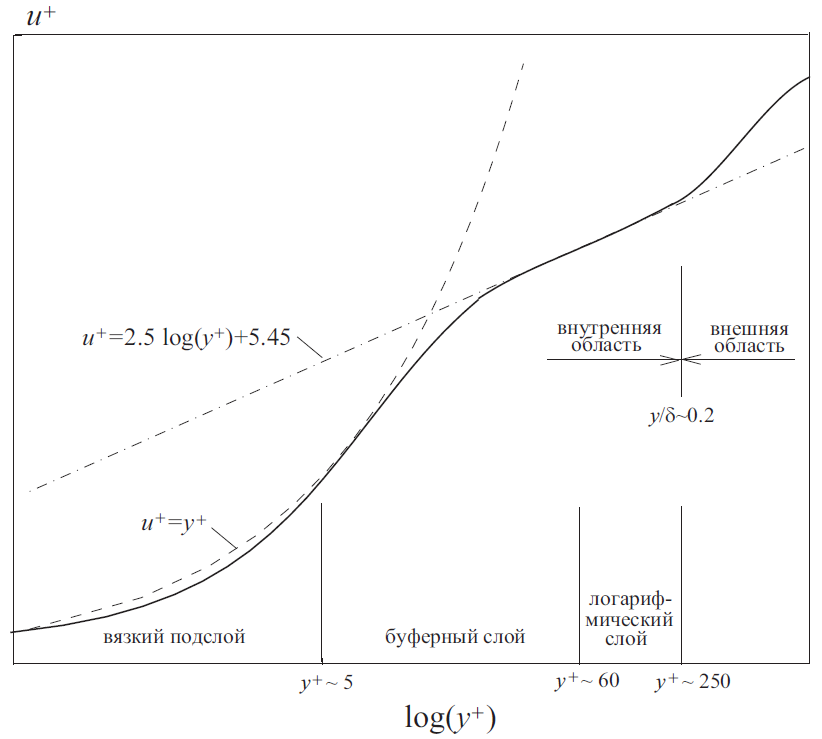
\includegraphics[width=0.7\linewidth]{../Assets/ПогранСлой}
		\caption{Схема слоя}
	\end{figure}
		
		Турбулентный пограничный слой разделяется на две области: внешняя и внутрення. Внутренняя область пограничного слоя занимает примерно 20\% от толщины всего слоя и в ней генерируется до 80\% энергии турбулентности.
		
	\subsubsection{Внешняя область}
		
		Внешний слой является областью полностью развитого турбулентного течения, в котором распределение скорости описывается логарифмическим законом. Полное затухание возмущений во внешней области происходит на расстоянии, во много раз превышающем линейный масштаб турбулентности.
		
		Чтобы определить поток во внешней зоне, применяют фильтрованные или усредненные по Рейнольдсу уравнения Навье-Стокса. В то же время, профиль скорости во внутренней зоне сравнительно мало зависит от различных внешних условий, таких как числа Рейнольдса и градиент давления, что позволяет использовать универсальные соотношения (пристеночные функции) для связи параметров потока с расстоянием от стенки. Этот метод также базируется на гипотезе о локальном равновесии энергии турбулентных пульсаций и свойствах локальной изотропности диссипирующих вихрей.
		
	\subsubsection{Внутрення область}
	
		Вязкий подслой, буферный и логарифмический слои составляют внутреннюю область пограничного слоя. Она характеризуется высокой скоростью переноса массы, импульса и тепла, что приводит к повышенной трению и потере энергии.
		
		Существует два подхода к моделированию течения в пристеночной области. В первом подходе используются полуэмпирические формулы (пристеночные функции) для описания внутреннего слоя потока, в то время как во втором подходе модели турбулентности модифицируются таким образом, чтобы разрешать всю пристеночную область потока, включая вязкий подслой, при условии обеспечения необходимого разрешения сетки в пограничном слое. Такие модели турбулентности могут быть использованы для расчета турбулентных течений во всей расчетной области (включая пристеночную область течения).
		
	\subsubsection{Свойства пограничного слоя}
	
		Толщина пограничного слоя трудно определима как в расчёте, так и в эксперименте. Для определения используются понятия: толщина вытеснения $\delta^*$ и толщина потери импульса $\theta$.
		\begin{equation}
			\delta^* = \int_{0}^{\infty}(1 - \frac{u}{U_e})dy \qquad \theta = \delta^{**} = \int_{0}^{\infty} \frac{u}{U_e}(1 - \frac{u}{U_e})dy
		\end{equation}
		Кроме того используется безразмерный параметр $H$:
		\begin{equation}
			H = \frac{\delta^*}{\theta}
		\end{equation}
		 
		Число Рейнольдса характеризуется двумя величинами($Re_x$ и $Re_\theta$): расстоянием от начала $x$ и толщиной $\theta$.
		\begin{equation}
			Re_x = \frac{xU_e}{\nu} \qquad Re_\theta = \frac{\theta U_e}{\nu}
		\end{equation}
		 
		Используя напряжение трения на стенке $\tau_w$ можем вычислить коэффициент трения $C_F$ и динамическую скорость $v^*$:
		\begin{equation}
			\tau_w = v\frac{\partial u}{\partial y}\bigg|_W \qquad C_F = \frac{\tau_w}{0.5\rho U_e^2} \qquad v^* = \sqrt{\frac{\tau_w}{\rho}}
		\end{equation}
	 
		Не менее важной характеристикой пограничных слоев является продольный градиент давления:
		\begin{equation}
			\frac{dp}{dx} = -\rho U_e \frac{dU_e}{dx}
		\end{equation}
		 
		Часто на пограничные слои влияют такие факторы: кривизна поверхности $\kappa$, скорость закачки и откачки жидкости(газа), шероховатость поверхности $k_s^+$(высота бугорков).
		\begin{equation}
		 	\kappa = \frac{\delta^*}{R} \qquad \frac{V_W}{v^*}, \frac{V_W}{U_e} \qquad k_s^+ = \frac{k_s v^*}{\nu}
		\end{equation}
	 	
	 	Важным свойством пограничного слоя является выполнение интегрального уравнения импульсов. Верно и обратное: если уравнение импульсов не выполняется, то уравнения плоского пограничного слоя также не верны для этого течения. Это может быть обусловлено разными причинами: трехмерность течения, его нестационарность, влияние вверх по потоку, изменение давления поперек пограничного слоя, влияние нормальных Рейнольдсовых напряжений и т.д.
	 	\begin{equation}
	 		\frac{d\theta}{dx} + \frac{dU_e}{dx}\cdot\frac{2 + H}{U_e}\theta - \frac{C_f}{2} = 0
	 	\end{equation}
		 
	\subsection{Турбулентное состояние пограничного слоя}
	‍
		Турбулентное движение в пограничном слое возникает из-за нестабильности потока, которая проявляется в виде вихрей различных размеров и интенсивности. Эти вихри перемешивают слои жидкости или газа, что приводит к увеличению переноса массы и энергии вдоль поверхности твердого тела. Параметры турбулентного потока в пограничном слое характеризуются такими величинами, как скорость, давление, плотность и температура. Важными параметрами являются также коэффициент трения, переноса тепла и массы. Турбулентное течение с большим числом Рейнольдса называют развитой турбулентностью.
		
		Для описания турбулентности используются уравнения Навье-Стокса, которые описывают законы сохранения массы, импульса и энергии для жидкости. Однако аналитическое решение этих уравнений возможно только для очень простых течений. В общем случае для описания турбулентных потоков применяются численные методы, такие как метод прямого численного моделирования или моделирование крупных вихрей. Одной из фундаментальных проблем гидродинамики турбулентных течений является проблема турбулентного переноса. Она связана с необходимостью описать перемещение частиц жидкости и массы, энергии и импульса в условиях сложных турбулентных потоков
		
		Существует каскадный перенос энергии, т.е. её передача от более крупных вихрей к более мелким. Наиболее крупные вихри получают энергию от осредненного течения, передают её всё более мелким, а наиболее мелкие диссипируют в тепло. Скорость этого процесса в силу хаотичности природы турбулентности также колеблется вокруг некой величины, при этом ее мгновенное значение может становиться отрицательным. Иными словами, в некоторые моменты времени энергия может передаваться от более мелких вихрей к более крупным, но эта флуктуация компенсируется более интенсивной передачей энергии по каскаду в другие моменты времени.
		
	\subsection{Локальное трение и перенос}
		% Тут надо ещё подумать почитать и переделать %
		Локальное трение - это сопротивление движению тела, возникающее при контакте поверхностей, на которых оно скользит. В отличие от идеального или нулевого трения, локальное трение всегда присутствует в реальных условиях. Перенос же - это процесс перемещения чего-либо из одного места в другое. Локальное трение может оказывать влияние на перенос. Например, если объект движется по поверхности, на которой есть локальное трение, то его движение замедляется и потеря энергии происходит за счет трения. Это может привести к тому, что объект не сможет полностью передать свою энергию и импульс другому объекту при столкновении, так как часть энергии будет потеряна на трение.
		
	\subsection{Методы моделирования}
	
		Несмотря на интенсивное развитие вычислительной техники и впечатляющие успехи, достигнутые в последние годы как в области построения эффективных численных алгоритмов, предназначенных для решения задач гидромеханики и тепломассопереноса, так и в разработке сопутствующего математического обеспечения (генераторы сеток, интерактивные системы ввода данных и систем визуализации результатов расчетов), проблема численного моделирования турбулентности, как и на протяжении многих предшествующих десятилетий, по-прежнему остается одной из наиболее сложных и актуальных проблем механики жидкостей. В отличие от ламинарных течений однофазной среды (жидкости или газа), расчет которых, благодаря отмеченным выше достижениям, стал во многом рутинной процедурой, надежное предсказание характеристик сложных турбулентных течений, представляющих наибольший практический интерес все еще остается сложным.
	
		Выбор модели турбулентности зависит от характера турбулентного потока, требуемой точности, доступных вычислительных ресурсов и временных затрат. Выбор подходящей модели турбулентности для решение конкретной задачи требует четких представлений свойств и ограничений каждой модели турбулентности. Для моделирования нестационарных течений возможно использовать несколько принципиально различных вычислительных и физических подходов:
		\begin{enumerate}
			\item Использование моделей турбулентности, обеспечивающих достаточно точное предсказание измеряемых в эксперименте осредненных параметров потока в рамках стационарных уравнений Рейнольдса.
			\item Использование нестационарных уравнений Рейнольдса в сочетании с условиями симметрии, что приводит к симметричным нестационарным решениям.
			\item Использование нестационарных уравнений Рейнольдса в сочетании с традиционными полуэмпирическими моделями турбулентности без привлечения условий симметрии.
		\end{enumerate}
	
	\subsubsection{DNS}
	
		Прямое численное моделирование(DNS) предполагает решение полных нестационарных трехмерных уравнений Навье-Стокса, позволяющее получить мгновенные характеристики турбулентного потока. Проблемы, связанные с широким использованием DNS связаны с высокими требованиями к используемой разностной схеме, удовлетворением начальных и граничных условий, а также ограниченными ресурсами вычислительной техники. Расчетная область при этом должна быть достаточно протяженной, чтобы вместить наибольшие масштабы турбулентности, а шаг интегрирования по времени должен иметь порядок колмогоровского масштаба времени.
		
		\begin{table}[H]
			\begin{center}
				\begin{tabular}{|c|c|c|c|c|}
					\hline
					Re & 6.6$\times10^3$ & 2.0$\times10^4$ & 1.0$\times10^5$ & 1.0$\times10^6$\\
					\hline
					Кол-во узлов сетки & 2$\times10^6$ & 4$\times10^7$ & 3$\times10^8$ & 1.5$\times10^3$\\
					\hline
					150 MFlops & 37 ч & 740 ч & 6.5 лет & 3000 лет\\
					\hline
					1 TFlops & 20 с & 400 с & 8.3 ч & 4000 ч\\
					\hline
				\end{tabular}
			\end{center}
			\caption{Затраты времени при различных параметрах}
		\end{table}
	
	\subsubsection{RANS}
	
		В инженерных приложениях широко используются математические модели, основанные на численном решении осредненных по Рейнольдсу уравнений Навье-Стокса(RANS). При использовании уравнений Рейнольдса основной интерес проявляется к динамике крупномасштабных вихрей, ответственных за переносные свойства турбулентных течений. При замыкании уравнений Рейнольдса рассматриваются масштабы длины, типичные для энергосодержащих вихрей, в которых $Re\gg1$ (за исключением пристеночных областей). Для учета пристеночного влияния диссипирующих вихрей и энергосодержащих вихрей при $Re\sim1$ используются демпфирующие функции.
		
		Уравнения Навье-Стокса:
		\begin{equation}
			\begin{cases}
				\frac{\partial u_i}{\partial x_i} = 0
				\\
				\rho\frac{\partial u_i}{\partial t} + \rho u_j \frac{\partial u_i}{\partial x_j} = - \frac{\partial p}{\partial x_i} + \frac{\partial}{\partial x_j}(\mu\frac{\partial u_i}{\partial x_j})
			\end{cases}
		\end{equation}
		
			
	\subsubsection{LES}
	
		Метод моделирования крупных вихрей(LES) был предложен Иосифом Смагоринским в 1963 году. Он основан на двух предположениях. Первый предполагает, что течение можно разделить на движение крупных и мелких вихрей. Крупные вихри, находящиеся под прямым воздействием граничных условий и несущие в себе максимум рейнольдсовых напряжений, рассчитываются. Мелкомасштабная турбулентность считается изотропной и имеющей универсальные характеристики, а потому менее критичной и более поддающейся моделированию. Другой  заключается в возможности аппроксимации нелинейных взаимодействий между крупными и мелкими вихрями только по крупным вихрям с использованием подсеточных моделей(SGS). Иначе говоря, принимается гипотеза о статистической независимости крупных и мелких вихрей.
	
		Статистика крупных вихрей обычно не чувствительна к подсеточному моделированию за исключением пристеночной области. Имеющиеся подсеточные модели корректно предсказывают не только осредненные характеристики потока (первые и вторые моменты), но также и флуктуации интегральных характеристик, например, коэффициентов сопротивления и подъемной силы\cite{Fureby2000}.
	
		Мелкомасштабное движение исключается из уравнений Навье-Стокса при помощи применения операции фильтрации и моделируются с помощью подсеточных моделей. На рисунке \ref{fig:lesfilter} показан принцип работы фильтров, где $f(x)$ - исходный вариант, $\tilde{f}(x)$ - после фильтрации.\\
		\begin{figure}[H]
			\centering
			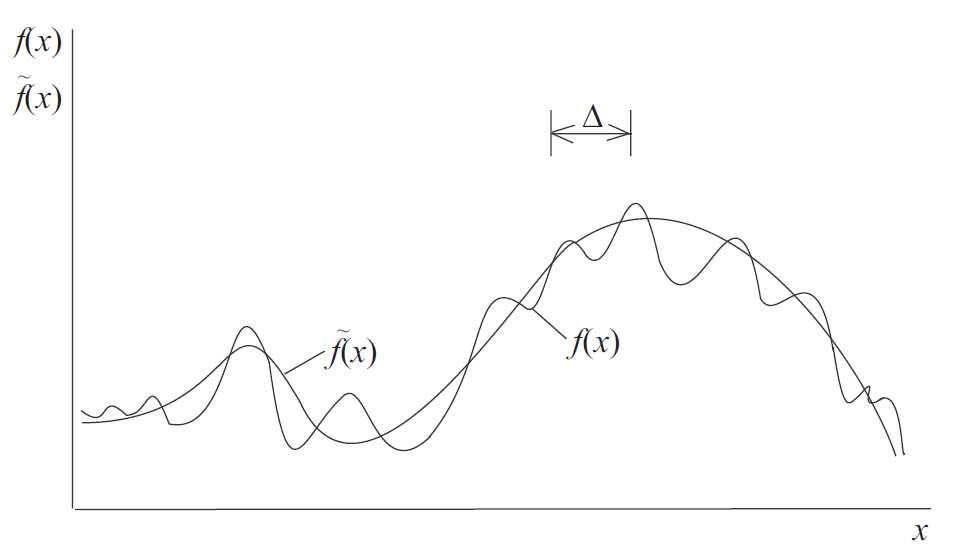
\includegraphics[width=0.7\linewidth]{../Assets/ФильтрацияLES}
			\caption{Исключение мелкомасштабных движений фильтрацией}
			\label{fig:lesfilter}
		\end{figure}
	
		Уравнение фильтра, применимое к пространственно временному полю $\phi(x,t)$ представлено ниже:
		\begin{equation}
			\overline{\phi(x,t)} = \int_{-\infty}^{\infty}\int_{-\infty}^{\infty}\phi(r,t')G(x - r, t - t')dt'dr
		\end{equation}
		В данном случае $G$ - ядро, характерное для каждого типа фильтра.
	
		Решение, полученное с помощью LES, содержит более богатую информацию по сравнению с решением на основе уравнений Рейнольдса, например, не только характеристики среднего течения (поля скорости, концентрации, температуры, давления) и распределения рейнольдсовых напряжений, но также и спектральные характеристики (спектры пульсаций скорости и давления), двухточечные моменты, временные и пространственные масштабы турбулентности.
	
	\subsubsection{DES}
	
		Характерные для отрывных течений крупномасштабные нестационарные трехмерные вихревые структуры определяются конкретными граничными условиями и геометрическими характеристиками рассматриваемых течений и не могут быть описаны в рамках таких моделей. Это стимулируют поиск и разработку гибридных подходов, сочетающих в себе экономичность RANS и универсальность LES.
		
		В методе моделирования отсоединенных вихрей (DES) в области присоединенного пограничного слоя метод функционирует в режиме уравнений Рейнольдса, а в области отрыва потока переходит в LES. При этом достигается сочетание лучших качеств обоих подходов -- высокая точность и экономичность уравнений Рейнольдса в области присоединенного пограничного слоя и универсальность LES в отрывной области. Хотя DES, в отличие от RANS, является принципиально нестационарным трехмерным подходом, необходимые для его реализации сетки в пристеночной области совпадают с сетками, необходимыми для решения уравнений Рейнольдса, и являются на много порядков меньшими, чем сетки, требуемые для разрешения мелких пристенных вихрей в рамках LES. По мере измельчения сетки DES асимптотически приближается к LES и далее к DNS. Конкретные реализации DES основаны на использовании модели турбулентной вязкости Спаларта-Аллмареса и модели Ментера\cite{Strelets2001}.
	
	\subsubsection{Оценка производительности}
	
	Оценка количества узлов сетки и временных шагов, необходимых для реализации DNS и LES, показывает сложность проблемы с вычислительной точки зрения.
	
	\begin{table}[H]
		\begin{center}
			\begin{tabular}{|c|c|c|c|c|}
				\hline
				Метод & Число узлов сетки & Число шагов по времени & Готовность\\
				\hline
				RANS & $10^7$ & $10^3$ & 1985\\
				\hline
				DES & $10^8$ & $10^4$ & 2000\\
				\hline
				LES & $10^{11.5}$ & $10^{6.7}$ & 2045\\
				\hline
				DNS & $10^{16}$ & $10^{7.7}$ & 2080\\
				\hline
			\end{tabular}
		\end{center}
		\caption{Перспектива применения методов}
	\end{table}
	Готовность означает практическое применение метода с затратой времени не более суток.
	
	\numsection{Глава 2}
	\subsection{Постановка задачи}
	\subsection{Визуализация поставленной задачи}
	\subsubsection{Геометрия канала}
		% Перефразировать или более красивое описание %
		Прямоугольный канал, сужающийся от 369.5$\times$149.8 мм вначале канала до 124$\times$50 мм на расстоянии 396 мм от начала канала. На расстоянии 323.9 мм от начала канала находится искусственное препятствие, представляющее собой вырез, имитирующий проволоку радиусом 2.1 мм и высотой 1.98 мм. Длина прямого участка канала 1100 мм.
		
		\begin{figure}[H]
			\centering
			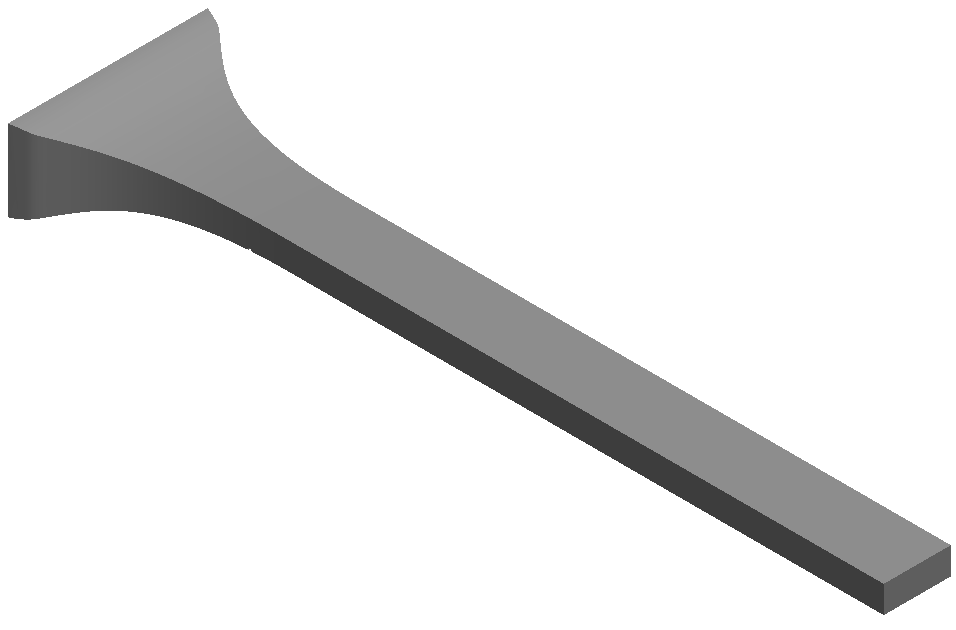
\includegraphics[width=0.7\linewidth]{../Assets/ВидКанала1}
			\caption{Вид канала}
			\label{fig:channelview}
		\end{figure}
		
	\subsubsection{Построение сеточной модели}
		% Описать построение сетки, способы и про оптимизацию + схема из отчёта + вся статистика сетки %
		Существует несколько методов моделирования сеточных моделей в Ansys, которые можно использовать в зависимости от типа и размера модели.
		
		Один из методов -- это метод пространственного разбиения, который часто используется для моделирования твердых тел. Этот метод заключается в разбиении объекта на более мелкие элементы, называемые конечными элементами. Затем каждый конечный элемент аппроксимируется более простыми формами, такими как треугольники или прямоугольники, чтобы создать сетку.
		
		Второй -- это метод генерации сетки на основе узлов. В этом методе модель представляется в виде набора узлов, соединенных линиями или поверхностями. Затем сетка строится на основе этой структуры.
		
		Третий -- это метод многократного разделения. Этот метод часто используется для моделирования пространственных объектов, таких как воздушные суда или автомобили. Он заключается в разбиении объекта на более мелкие блоки и последующем разделении каждого блока на еще более мелкие блоки. Затем каждый блок аппроксимируется более простыми формами для создания сетки.
	
		\begin{figure}[H]
			\centering
			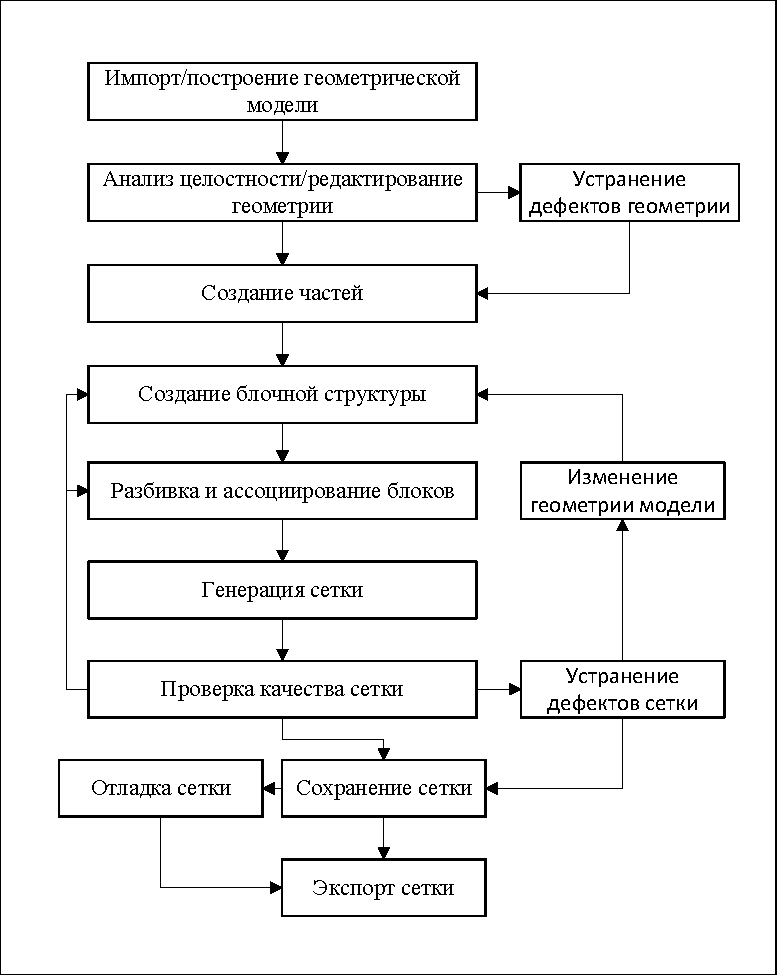
\includegraphics[width=0.8\linewidth]{../Assets/СхемаСозданияСетки}
			\caption{Схема работы над сеточной моделью}
			\label{fig:meshScheme}
		\end{figure}
	
	\subsection{Вычисление в ANSYS Fluent}
	% Тут про настройки fluent и куча его параметров при запуске вычислений %
	\numsection{Глава 3}
	\subsection{Анализ полученных результатов}
	\subsection{Влияние на локальное трение и перенос}
	\anonsection{Заключение}
	\newpage
	\addcontentsline{toc}{section}{Список использованных источников}
	\bibliography{bibliography}
\end{document}